\documentclass[010-intro.tex]{subfiles}

\begin{document}

    \subsection{Communities in Data Science History: The Carpentries}

        Programming is not a taught in many academic disciplines.
        But as research relied more on computational tools,
        a growing need for teaching and learning these computational tools in academia was needed.

        Software Carpentry was founded in 1998 by Greg Wilson and Brent Gorda with the goal of
        teaching researchers the computing skills to get their work done more efficiently and effectively.
        These workshops are primarily focused on general programming skills for scientific computation,
        and were made open source in 2005 with support from the Python Software Foundation (PSF).
        Software Carpentry continues to grow with the support from the Alfred P. Sloan Foundation and Mozilla Science Lab in 2012
        \cite{CarpentriesHowWe, jordanCarpentries2020Annual}.

        % and NumFOCUS was also founded as a 501(c)(3) public charity status as a nonprofit in the United States with the mission to support open source projects and help sustain them.

        The following year, 2013, the first workshops geared towards Librarians were run.
        By 2014, Data Carpentry is founded by Karen Cranston, Hilmar Lapp, Tracy Teal, and Ethan White
        with support from the National Science Foundation (NSF)
        with the goal of creating materials focused on data literacy aimed at novices in specific research domains.
        James Baker is able to expand on Library Carpentry with support from the Software Sustainability Institute (SSI)
        with the goal of teaching information sciences and best practices in data structures.
        Software Carpentry Foundation is also founded under NumFOCUS in 2014.
        In 2015, Data Carpentry gets support from the Gordon and Betty Moore Foundation and
        in 2018, with the help of Community Initiatives, Software Carpentry, Data Carpentry, and Library Carpentry
        merge together to form The Carpentries.
        From 2012 to 2020, The Carpentries have run
        2,700 workshops across 71 countries and have touched at least 66,000 novice learners
        \cite{CarpentriesHowWe, jordanCarpentries2020Annual}.

        Today, the Carpentries support over 50 lessons across their 3 Lesson Programs
        (Data Carpentry, Library Carpentry, and Software Carpentry),
        with over 150 lesson maintainers
        \cite{chenPointContactEach}.
        These lessons cover all the basic data literacy, data management, data science, and software programming
        skills in specific curricula domains (Figure \ref{fig:carpentries-venn}).
        Instead of having one-off lesson materials maintained by a small set of authors,
        The Carpentries lessons are kept up-to-date with a rotating set of maintainers for each lesson,
        and leverage the broader community to upkeep the teaching infrastructure.


        \begin{figure}[htb]
            \centering
            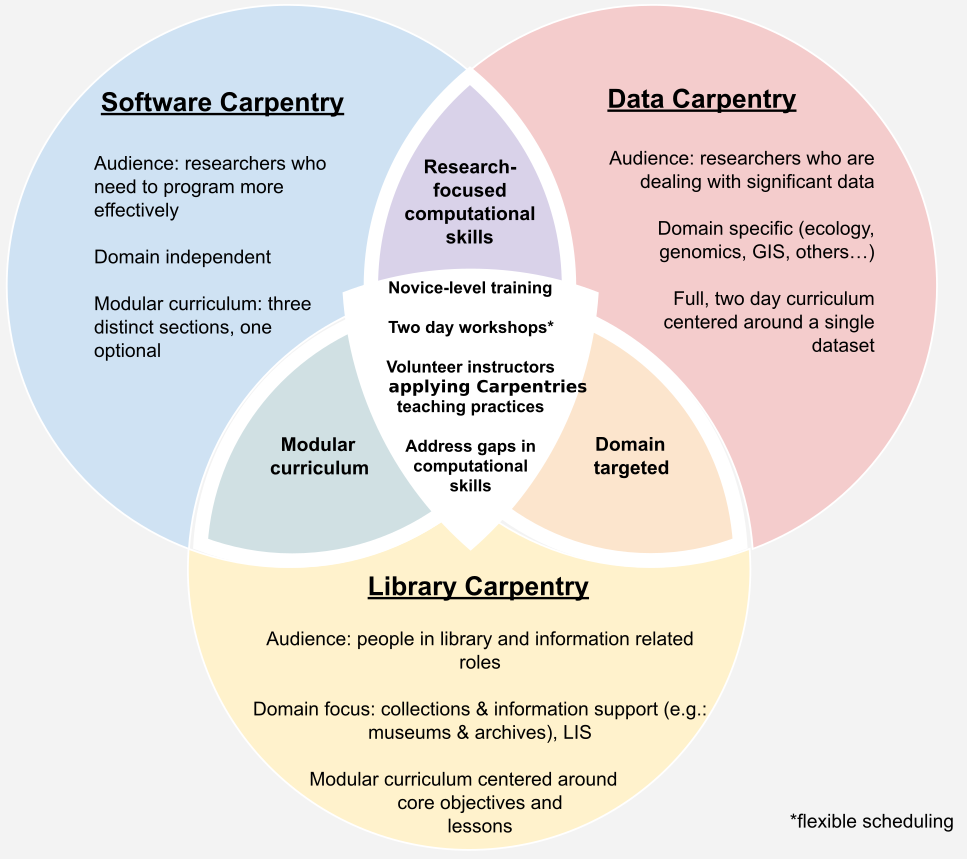
\includegraphics[scale=0.5]{figs/050-intro/carpentries-venn}
            \caption[Differences between Carpentries Lesson programs]{
            The differences between the 3 Carpentries lesson programs: Data Carpentry, Library Carpentry, and Software Carpentry.
            Data Carpentry focuses more on researchers who work with data in a specific domain,
            Library Carpentry focuses more on programming tasks in the library and information sciences, and
            Software Carpentry focuses more on programming concepts.
            Figure adapted from the Carpentries Trainer Training lesson \cite{CarpentryTrainerTraining}.
            }
            \label{fig:carpentries-venn}
        \end{figure}


\end{document}
